 % The main file for CAMP reports
 % Don't put any content in here. 
 % Don't even include content files by using \input or \inlcude. 
 % Put your content to TEXT.TEX or include it there using \input.
 % Uses:
 %		SETTINGS.TEX		contains the settings for this document
 %		COMMANDS.TEX		contains commands which can be used while writing
 %		INFO.TEX			contains the author, title and so on for the cover
 %		COVER.TEX			formats the front cover of the document
 %		ABSTRACT.TEX		contains the abstract to be included (if needed)
 %		TEXT.TEX			contains the actual content of the document
 %		BIB.BIB				containt the BibTeX entries for the document
 


%% Draft document mode
%% Final document
%\documentclass[11pt,a4paper,bibtotoc,idxtotoc,headsepline,footsepline,footexclude,BCOR15mm,DIV13]{scrbook}
\documentclass[11pt,a4paper,bibtotoc,idxtotoc,headsepline,footsepline,footexclude,DIV13,oneside]{scrbook}

%\documentclass[11pt,a4paper,bibtotoc,idxtotoc,headsepline,footsepline,footexclude,BCOR20mm,DIV10]{scrbook}

%\usepackage{epstopdf}
% KOMA-Optionen:
%  bibtotoc: include bibliography in table of contents
%  idxtotoc: include index in table of contents
%  headsepline: use horizontalline under heading
%  BCOR: binding correcion (Bindungskorrektur) (e.g.: BCOR5mm)
%  DIV: Number of sheet sections (used for layout) (e.g.: DIV12) 



% include title and author information for the cover
% Set here the title, authors and other stuff to be used for the cover
% This file is used by MAIN.TEX

% set title, authors and stuff for the cover
\def\doctype{BGCE Honours project report}
\def\title{CAD-integrated Topology Optimization}
\def\titleGer{CAD-integrierte Optimisierung von Topologie}
\def\author{S. Joshi, J.C. Medina, F. Menhorn, S. Reiz, B. Rüth, E. Wannerberg, A. Yurova}
\def\date{\today}

% text to appear in the footer
\def\footertext{}

% include settings
% Included by MAIN.TEX
% Defines the settings for the CAMP report document

\renewcommand{\sectfont}{\normalfont \bfseries}        % Schriftart der Kopfzeile

% manipulate footer
\usepackage{scrpage2}
\pagestyle{scrheadings}
\ifoot[\footertext]{\footertext} % \footertext set in INFO.TEX
%\setkomafont{pagehead}{\normalfont\rmfamily}
\setkomafont{pagenumber}{\normalfont\rmfamily}

%% allow sophisticated control structures
\usepackage{ifthen}

% use Palatino as default font
\usepackage{palatino}

% enable special PostScript fonts
\usepackage{pifont}

% make thumbnails
\usepackage{thumbpdf}

%to use the subfigures
\usepackage{subcaption}

\usepackage{colortbl}
\usepackage{color}
\definecolor{Gray}{gray}{0.9}

%for high quality horizontal lines
\usepackage{booktabs}

%% show program code\ldots
%\usepackage{verbatim}
%\usepackage{program}

%% enable TUM symbols on title page
\usepackage{styles/tumlogo}


\usepackage{multirow}

%% use colors
\usepackage{color}

%% make fancy math
\usepackage{amsmath}
\usepackage{amsfonts}
\usepackage{amssymb}
\usepackage{units}
\usepackage{textcomp}
\usepackage{yhmath} % fr die adots 
%% mark text as preliminary
%\usepackage[draft,german,scrtime]{prelim2e}

\usepackage{url}

%% create an index
\usepackage{makeidx}

% for the program environment
\usepackage{float}

%% load german babel package for german abstract
%\usepackage[german,american]{babel}
\usepackage[german,english]{babel}
\selectlanguage{english}

% use german characters as well
\usepackage[latin1]{inputenc}       % allow Latin1 characters

% use initals dropped caps - doesn't work with PDF
%\usepackage{dropping}
 %\usepackage[dvips]{dropping}

\usepackage{styles/shortoverview}
%----------------------------------------------------
%      Graphics and Hyperlinks
%----------------------------------------------------

%% check for pdfTeX
\ifx\pdftexversion\undefined
 %% use PostScript graphics
 \usepackage[dvips]{graphicx}

 \DeclareGraphicsExtensions{.eps,.epsi}
 \graphicspath{{figures/}{figures/review}{Pictures/}} 
 %% allow rotations
 \usepackage{rotating}
 %% mark pages as draft copies
 %\usepackage[english,all,light]{draftcopy}
 %% use hypertex version of hyperref
 \usepackage[hypertex,hyperindex=false,colorlinks=false]{hyperref}
\else %% reduce output size \pdfcompresslevel=9
 %% declare pdfinfo
 %\pdfinfo { 
 %  /Title (my title) 
 %  /Creator (pdfLaTeX) 
 %  /Author (my name) 
 %  /Subject (my subject	) 
 %  /Keywords (my keywords)
 %}
 %% use pdf or jpg graphics
 \usepackage[pdftex]{graphicx}
 \DeclareGraphicsExtensions{.jpg,.JPG,.png,.pdf,.eps}
 \graphicspath{{figures/}{Pictures/}} 
 
 %% Load float package, for enabling floating extensions
 \usepackage{float}
 
% \usepackage{mdframed}
 
 %% allow rotations
 \usepackage{rotating}
 %% use pdftex version of hyperref
 \usepackage[pdftex,pdfauthor={Joshi, Saumitra; Medina, Juan Carlos; Menhorn, Friedrich; Reiz, Severin; R{\"u}th, Benjamin; Wannerberg, Erik; Yurova, Anna},%
            pdftitle={CAD-integrated Topology Optimization},%
%            pdfsubject={The Subject},
            pdfkeywords={Topology Optimization, CAD description generation, CAD-integrated topology optimization},%
            colorlinks=true,linkcolor=black,citecolor=red,%
 anchorcolor=red,urlcolor=blue,bookmarks=true,%
 bookmarksopen=true,bookmarksopenlevel=0,plainpages=false%
 bookmarksnumbered=true,hyperindex=false,pdfstartview=%
 ]{hyperref}
%
%\usepackage[pdftex,colorlinks=false,linkcolor=red,citecolor=red,%
% anchorcolor=red,urlcolor=red,bookmarks=true,%
% bookmarksopen=true,bookmarksopenlevel=0,plainpages=false%
% bookmarksnumbered=true,hyperindex=false,pdfstartview=%
% ]{hyperref}
\fi
\usepackage{epstopdf}
\epstopdfsetup{update} % only regenerate pdf files when eps file is newer

\usepackage{listings} %source code formatter
%\usepackage{courier}

\lstset{basicstyle=\ttfamily,breaklines=true}
\lstset{framextopmargin=50pt,frame=bottomline}

% package for notes
\usepackage[obeyFinal, colorinlistoftodos]{todonotes}

% for comments
\usepackage{verbatim}

% package for acronyms
\usepackage{acro}

% for fancy tabulars
\usepackage{tabularx}

% for itemize and enum extensions
\usepackage{enumitem}

%% Fancy chapters
%\usepackage[Lenny]{fncychap}
%\usepackage[Glenn]{fncychap}
%\usepackage[Bjarne]{fncychap}

%\usepackage[avantgarde]{quotchap}

% set the bibliography style
%\bibliographystyle{styles/bauermaNum}
%\bibliographystyle{alpha}
\bibliographystyle{unsrt}

% for striking out sentences
\usepackage{soul}


% include commands
% Commands to be used within the TUM report document
% Included by MAIN.TEX
% Please include your own cool commands here. 
% Be only sure to comment it sufficiently so others can use it.

%-------------------------------------------------------------
%                      Own Commands
%-------------------------------------------------------------


%-------------------------------------------------------------
% math stuff -------------------------------------------------

% nice R, N, C
\newcommand{\nat}{\mathbb{N}}
\newcommand{\real}{\mathbb{R}}
\newcommand{\compl}{\mathbb{C}}


\newcommand{\dx}{\text{d}x}
\newcommand{\dt}{\text{d}t}
\newcommand{\du}{\text{d}u}
\newcommand{\dv}{\text{d}v}
\newcommand{\where}{\text{where}}

% norm
\newcommand{\norm}[1]{\left\| #1 \right\|}
\newcommand{\Ltwonorm}[1]{\norm{#1}_{L_2}}

% un demi
\newcommand{\half}{\frac{1}{2}}

% parantheses
\newcommand{\parenth}[1]{ \left( #1 \right) }
\newcommand{\bracket}[1]{ \left[ #1 \right] }
\newcommand{\accolade}[1]{ \left\{ #1 \right\} }
%\newcommand{\angle}[1]{ \left\langle  #1 \right\rangle }

% partial derivative: %#1 function, #2 which variable
% simple / single line version
\newcommand{\pardevS}[2]{ \delta_{#1} f(#2) }
% fraction version
\newcommand{\pardevF}[2]{ \frac{\partial #1}{\partial #2} }

% render vectors: 3 and 4 dimensional
\newcommand{\veciii}[3]{\left[ \begin{array}[h]{c} #1 \\ #2 \\ #3	\end{array} \right]}
\newcommand{\veciv}[4]{\left[ \begin{array}[h]{c} #1 \\ #2 \\ #3 \\ #4	\end{array} \right]}

% render matrices: 3  dimensional (arguments in row first order)
\newcommand{\matiii}[9]{\left[ \begin{array}[h]{ccc} #1 & #2 & #3 \\ #4 & #5 & #6 \\ #7 & #8 & #9	\end{array} \right]}
%DOESN'T WORK,DON'T KNOW WHY \newcommand{\mativ}[16]{\left[ \begin{array}[h]{cccc} #1 & #2 & #3 & #4 \\ #5 & #6 & #7 & #8 \\ #9 & #10 & #11 & #12 \\ #13 & #14 & #15 & #16 \end{array} \right]}




%-------------------------------------------------------------
% some peters' nomenclature ----------------------------------
\renewcommand{\vec}[1]{\mathbf{#1}}
\newcommand{\petersPatchPoint}{V}
\newcommand{\petersPatchPoints}{\petersPatchPoint_x}
\newcommand{\petersControlMesh}{M}
\newcommand{\petersControlMeshRef}{\petersControlMesh_{ref}}
\newcommand{\petersControlMeshDobRef}{\petersControlMesh_{2ref}}
\newcommand{\petersControlMeshVec}{\vec{\MakeLowercase{\petersControlMesh}}}
\newcommand{\petersPatchPointVec}{\vec{\MakeLowercase{\petersPatchPoint}}}
\newcommand{\petersPatchPointMatrix}{\MakeUppercase{\petersPatchPoint}}
\newcommand{\petersLocalPatchPointLetter}{B}
\newcommand{\petersLocalPatchPoint}{\vec{\petersLocalPatchPointLetter}^{\petersControlMesh}}
\newcommand{\petersLocalPatchPointIndices}[1]{\petersLocalPatchPoint_{#1}}
\newcommand{\petersControlPointCoefLetter}{c}
\newcommand{\petersControlPointCoef}{\petersControlPointCoefLetter^{PS}}
\newcommand{\petersControlPointCoefMatrix}{\MakeUppercase{\petersControlPointCoefLetter}^{PS}}
\newcommand{\bezierPoint}{P}
\newcommand{\bezierPointSet}{\bezierPoint_x}
\newcommand{\bezierPointVec}{\vec{\bezierPoint}}
\newcommand{\petersLocalBezPoint}{\vec{\petersLocalPatchPointLetter}^{\text{B{\'e}z}}}
\newcommand{\petersLocalBezPointIndices}[1]{\petersLocalBezPoint_{#1}}
\newcommand{\petersFaces}{F}
\newcommand{\suchthat}{;}
\newcommand{\centroidof}[1]{\vec{c}_{#1}}
\newcommand{\verticesof}[1]{V_{#1}}
\newcommand{\facesof}[1]{\petersFaces_{#1}}
\newcommand{\lsDataPointLetter}{D}
\newcommand{\lsDataPoint}{\vec{\MakeLowercase{\lsDataPointLetter}}}
\newcommand{\lsDataPointMatrix}{\MakeUppercase{\lsDataPointLetter}}
\newcommand{\lsDataPointConcMatrix}{\tilde{\lsDataPointMatrix}}
\newcommand{\lsControlPointLetter}{P}
\newcommand{\lsControlPointMatrix}{\MakeUppercase{\lsControlPointLetter}}
\newcommand{\lsControlPoint}{\vec{\MakeLowercase{\lsControlPointLetter}}}
\newcommand{\lsControlPointCoef}{c}
\newcommand{\lsControlPointCoefVec}{\vec{\lsControlPointCoef}}
\newcommand{\lsControlPointCoefMatrix}{\MakeUppercase{\lsControlPointCoef}}
\newcommand{\lsControlCoefConcMatrix}{\tilde{\lsControlPointCoefMatrix}}

\newcommand{\lsDataPointi}[1]{\lsDataPoint_{#1}}
\newcommand{\lsControlPointi}[1]{\lsControlPoint_{#1}}
\newcommand{\lsControlPointCoefi}[1]{\lsControlPointCoef_{#1}}


\newcommand{\Bez}{B{\'e}zier }
%-------------------------------------------------------------
% some abreviations ------------------------------------------
\newcommand{\Reg}{$^{\textregistered}$}
\newcommand{\reg}{$^{\textregistered}$ }
\newcommand{\Tm}{\texttrademark}
\newcommand{\tm}{\texttrademark~}
\newcommand {\bsl} {$\backslash$}

%-------------------------------------------------------------
%-------------------------------------------------------------


%-------------------------------------------------------------
% formating --------------------------------------------------

% Theorem & Co environments and counters
\newtheorem{theorem}{Theorem}[chapter]
\newtheorem{lemma}[theorem]{Lemma}
\newtheorem{corollary}[theorem]{Corollary}
\newtheorem{remark}[theorem]{Remark}
\newtheorem{definition}[theorem]{Definition}
\newtheorem{equat}[theorem]{Equation}
\newtheorem{example}[theorem]{Example}
\newtheorem{algorithm}[theorem]{Algorithm}

% inserting figures
\newcommand{\insertfigure}[4]{ % Filename, Caption, Label, Width percent of textwidth
	\begin{figure}[htbp]
		\begin{center}
			\includegraphics[width=#4\textwidth]{#1}
		\end{center}
		\vspace{-0.4cm}
		\caption{#2}
		\label{#3}
	\end{figure}
}

\newcommand{\insertfigureMISSING}[4]{ % Filename, Caption, Label, Width percent of textwidth
	\begin{figure}[htbp]
		\begin{center}
			\missingfigure{#1}
		\end{center}
		\vspace{-0.4cm}
		\caption{#2}
		\label{#3}
	\end{figure}
}




% referecing figures

\newcommand{\refFigure}[1]{ %label
	figure \ref{#1}
}
\newcommand{\refChapter}[1]{ %label
	chapter \ref{#1}
}

\newcommand{\refSection}[1]{ %label
	section \ref{#1}
}

\newcommand{\refParagraph}[1]{ %label
	paragraph \ref{#1}
}

\newcommand{\refEquation}[1]{ %label
	equation \ref{#1}
}

\newcommand{\refTable}[1]{ %label
	table \ref{#1}
}




\newcommand{\rigidTransform}[2]
{
	${}^{#2}\!\mathbf{H}_{#1}$
}

%code, in typewriter
\newcommand{\code}[1]
 {\texttt{#1}}

% page clearing
\newcommand{\clearemptydoublepage}{%
  \ifthenelse{\boolean{@twoside}}{\newpage{\pagestyle{empty}\cleardoublepage}}%
  {\clearpage}}


%-------------------------------------------------------------
%-------------------------------------------------------------


\newcommand{\etAl}{\emph{et al.}\mbox{ }}


\newcommand{\tododone}[2][noinline]{\todo[#1, color=green!40]{\textit{#2}}}
\newcommand{\todointern}[2][noinline]{\todo[#1, color=blue!40]{#2}}
\newcommand{\todointernal}{\todointern}
\newcommand{\todourgent}[2][noinline]{\todo[#1, color=red!40]{\textbf{#2}}}

% include acronyms and glossary
\acsetup{first-long-format=\itshape}

% class `abbrev': abbreviations:
\DeclareAcronym{DC}{
  short = DC ,
  long  = Dual Contouring ,
  class = abbrev
}
\DeclareAcronym{QEF}{
  short = QEF,
  long  = quadratic error function,
  class = abbrev
}
\DeclareAcronym{MC}{
  short = MC ,
  long  = Marching Cubes ,
  class = abbrev
}
\DeclareAcronym{DualMC}{
  short = DualMC ,
  long  = Dual Marching Cubes ,
  class = abbrev
}
\DeclareAcronym{DualMT}{
  short = DualMC ,
  long  = Dual Marching Tetrahedra ,
  class = abbrev
}
\DeclareAcronym{NURBS}{
  short = NURBS ,
  long  = Non-uniform Rational B-spline ,
  class = abbrev
}
\DeclareAcronym{Bspline}{
  short = B-spline ,
  long  = basis spline ,
  class = abbrev
}
\DeclareAcronym{CADTopOpt}{
  short = CADTopOpt,
  long = CAD-integrated Topology Optimization,
  class = abbrev
}
\DeclareAcronym{CAD}{
  short = CAD,
  long = Computer Aided Design,
  class = abbrev
}
\DeclareAcronym{CSG}{
  short = CSG,
  long = constructive solid geometry,
  class = abbrev
}
\DeclareAcronym{BREP}{
  short = BREP,
  long = boundary representation,
  class = abbrev
}
\DeclareAcronym{STL}{
  short = STL,
  long = stereo lithography,
  class = abbrev
}
\DeclareAcronym{STEP}{
  short = STEP,
  long = standard for the exchange of product model data,
  class = abbrev
}
\DeclareAcronym{IGES}{
  short = IGES,
  long = Initial Graphics Exchange Specification,
  class = abbrev
}
% class `nomencl': nomenclature
\DeclareAcronym{quad}{
  short = quad ,
  long  = quadrilateral face ,
  class = nomencl
}
\DeclareAcronym{tri}{
  short = triangle,
  long = triangular face,
  class = nomencl
}
\DeclareAcronym{patch}{
  short = patch,
  short-plural = es, 
  long  = a patch of rectangular topology,
  long-plural-form = patches of rectangular topology,
  class = nomencl
}
\DeclareAcronym{voxel}{
  short = voxel,
  long = a cube with uniform edge length and a datavalue on each corner of the cube,
  class = nomencl
}
\DeclareAcronym{Hermitedataone}{
  short = first order Hermite data,
  long = first derivative (gradient respectively) and value of a function at a certain point,
  class = nomencl
}


%\makeindex
	%% inter line spacing
%\linespread{1.0}

\makeglossary

\begin{document}

	\frontmatter
	
	
	%\input{components/cover}
%	\clearemptydoublepage
%	
%	% The titlepage for the CAMP report document.
% Included by MAIN.TEX


%--------------------------------------------------
% The title page
%--------------------------------------------------

% correct BCOR - undo at the end !!!
\def\bcorcor{0.15cm}
\addtolength{\hoffset}{\bcorcor}

\thispagestyle{empty}

 \vspace{10mm}
\begin{center}
	       %\oTUM{4cm}
	       
\includegraphics[width=4cm]{styles/tum_logo.png}
	   
	   \vspace{5mm}     
	   \huge Bavarian Graduate School of Computational Engineering \\Honours project\\ 
	   \vspace{0.5cm}
	 \large Technische Universit{\"a}t M{\"u}nchen\\
        
	\end{center}
		

\vspace{10mm}
\begin{center}

   {\Large \doctype}

  \vspace{10mm}
  
  {\LARGE \title}\\
  
  
  \vspace{10mm}
  
  
  %{\LARGE  \titleGer}\\
  
  
  %\vspace{10mm}

    %\hfill
    \begin{tabular}{ll}
	   \Large Authors:     & \Large \author \\[2mm]
%	   \Large $\mathrm{1^{st}}$ examiner:    & \Large Prof. Dr. However Wasit \\[2mm]				
%	   \Large $\mathrm{2^{nd}}$ examiner:    & \Large Prof. Dr. However Wasit \\[2mm]
	   \Large Advisors:    & \Large Arash, Dirk an Utz... \\[2mm]
%	   \Large Thesis handed in on:       & \Large August 15, 2006
	 \end{tabular}
	 
	 \vspace{5mm}
	 
	 \begin{figure}[h!]
  \centering
   \includegraphics[width=\textwidth]{styles/sccs_os2.pdf}
  \end{figure}
   

\end{center}

% undo BCOR correction
\addtolength{\hoffset}{\bcorcor}
	
	
%	\input{components/cover_maschmeyer}
	%\clearemptydoublepage
	
	% The titlepage for the CAMP report document.
% Included by MAIN.TEX


%--------------------------------------------------
% The title page
%--------------------------------------------------

% correct BCOR - undo at the end !!!
\def\bcorcor{0.15cm}
\addtolength{\hoffset}{\bcorcor}

\thispagestyle{empty}

 \vspace{10mm}
\begin{center}
	       %\oTUM{4cm}
	       
\includegraphics[width=4cm]{styles/tum_logo.png}
	   
	   \vspace{5mm}     
	   \huge Bavarian Graduate School of Computational Engineering \\Honours project\\ 
	   \vspace{0.5cm}
	 \large Technische Universit{\"a}t M{\"u}nchen\\
        
	\end{center}
		

\vspace{10mm}
\begin{center}

   {\Large \doctype}

  \vspace{10mm}
  
  {\LARGE \title}\\
  
  
  \vspace{10mm}
  
  
  %{\LARGE  \titleGer}\\
  
  
  %\vspace{10mm}

    %\hfill
    \begin{tabular}{ll}
	   \Large Authors:     & \Large \author \\[2mm]
%	   \Large $\mathrm{1^{st}}$ examiner:    & \Large Prof. Dr. However Wasit \\[2mm]				
%	   \Large $\mathrm{2^{nd}}$ examiner:    & \Large Prof. Dr. However Wasit \\[2mm]
	   \Large Advisors:    & \Large Arash, Dirk an Utz... \\[2mm]
%	   \Large Thesis handed in on:       & \Large August 15, 2006
	 \end{tabular}
	 
	 \vspace{5mm}
	 
	 \begin{figure}[h!]
  \centering
   \includegraphics[width=\textwidth]{styles/sccs_os2.pdf}
  \end{figure}
   

\end{center}

% undo BCOR correction
\addtolength{\hoffset}{\bcorcor}
	
	\clearemptydoublepage
\phantomsection
\addcontentsline{toc}{chapter}{Preface}	


\vspace*{3cm}

\begin{flushleft}
{\Large \bf Preface}
\end{flushleft}

\vspace{1cm}
The Bavarian Graduate School of Computational Engineering (BGCE) honours project at the Computational Science and Engineering (CSE) Institute of Technische Universit{\"a}t M{\"u}nchen (TUM) is a 10-month project where students conduct research on cutting-edge topics in the field of Computational Engineering, in cooperation with a partner in industry or academia. The 2015-16 project is titled \emph{CAD-Integrated Topology Optimization} and is initiated and supervised in a cooperation between TUM and Siemens AG in Munich.


\newpage

	
	%\input{components/disclaimer}
	
	\clearemptydoublepage
\phantomsection
\addcontentsline{toc}{chapter}{Acknowledgements}	


%\chapter*{Acknowledgements}

\vspace*{2cm}

\begin{center}
{\Large \bf Acknowledgments}
\end{center}

\vspace{1cm}




If someone contributed to the thesis... might be good to thank them here.
	
	%% Abstract for the TUM report document
% Included by MAIN.TEX

\clearemptydoublepage
\phantomsection
\addcontentsline{toc}{chapter}{Abstract}	





\vspace*{2cm}
\begin{center}
{\Large \bf Abstract}
\end{center}
\vspace{1cm}
In this document we provide the full guide on how to install CADO on Linux. We also provide installation instructions for all additional software used by CADO. All software used for the development of CADO and the CADO source code is open source.


	\tableofcontents
  	%outline and overview
   	\clearemptydoublepage

\phantomsection
\addcontentsline{toc}{chapter}{Outline and Overview of the document}

\begin{center}
	\huge{Outline and Overview}
\end{center}




%--------------------------------------------------------------------
The purpose of this document is to describe the implementation details of the \emph{CAD-integrated Topology Optimization} software tool along with the theoretical background it relies on. The document is arranged in chapters, covering introduction to the field and the project, background theory and parts of implementation. The chapters are described in more detail below.
\\
\\
%--------------------------------------------------------------------
\noindent {\scshape Chapter 1: Introduction}  \vspace{1mm}

\noindent  This chapter presents an overview of the motivation behind \emph{CAD-integrated Topology Optimization}, including the current state of the field. It also provides general organizational information about project execution, timeline and structure.
\\


%--------------------------------------------------------------------
\noindent {\scshape Chapter 2: Background Theory}  \vspace{1mm}

\noindent This chapter introduces the theoretical background for the implementation of the \emph{CAD-integrated Topology Optimization} tool. It consists of five parts, each describing essential background of the topology optimization pipeline. Furthermore, detailed description of selected algorithms used in each step is given.
\\

\noindent {\scshape Chapter 3: Implementation}  \vspace{1mm}

\noindent This chapter provides details on the implementation and structure of the \emph{CAD-integrated Topology Optimization} tool itself. The different parts of the topology optimization and surface-fitting pipeline are presented along with underlying implementation details.
\\ 

\noindent {\scshape Chapter 4: Results}  \vspace{1mm}

\noindent This chapter presents the implemented product of the \emph{CAD-integrated Topology Optimization} tool which the user experiences in terms of a graphical user interface. Additionally, three different test cases are described to show the performance of the integrated tool-chain.
\\

\noindent {\scshape Chapter 5: Summary and Future Work}  \vspace{1mm}

\noindent In the final chapter a summary of the whole project is provided. Weak spots of the algorithms are described including an outlook on areas where future optimization of the product is considered promising.  


\begin{comment}
\\
\noindent {\scshape Chapter 4: Summary and future work}  \vspace{1mm}

\noindent The final chapter summarizes the current status of the project and enumerates objectives for the next phase. \todourgent{Check if consistent with what the Gods want. -Saumi}
\\
\end{comment}
\tododone{Severin: Add chapter 4 and 5; Please proofread}


	\mainmatter
	
	
		% ---------------------------------------------------------------------------
		%
		%Introduction 
		%
		% ---------------------------------------------------------------------------
		\chapter{Introduction}
		\label{chapter:Introduction}
		\chapter{Introduction}
\label{chapter:Introduction}


 BGCE - who are we? moved to preface
\section{Motivation}


\section{Important concepts}

\subsection{Computer Aided Design - CAD}

\subsection{Topology Optimisation}

\section{Project structure}
\subsection{Aims and Goals}
\subsection{Timeline and Structure}

\section{Acknowledgement of supervisors}




		
		
		%
		%% ---------------------------------------------------------------------------
		%%
		%% and Background Theory
		%%
		%%% ---------------------------------------------------------------------------
		\chapter{Background Theory}
		\label{chapter:Background}
		\chapter{Background Theory}
\label{chapter:Background}

\section{CAD overview}
%interaction with it, programs, geometry represenations, datastructures, formats etc., maybe even history if we're overkill
\subsection{History of CAD}
Computer aided design (short: CAD) refers to the process of designing a product using a computer system. Before CAD applications were used, products were constructed using a sketch board. It was a challenge to incorporate changes in the construction drafts as well as to keep documentations up to date; hence, it was no surprise that CAD systems spread rapidly across all design development branches. Computer aided design is now irreplaceable used in architecture, mechanical, electrical and civil engineering.

Depending on the discipline different requirements are set on the virtual model. One may imagine that in a civil engineering model of a building a 2D floor plan is often sufficient; however in the design of a mechanical motor a 3D model is always necessary. Given these circumstances, various CAD software bundles evolved in the different disciplines with completely different modelling approaches. Besides the geometry representation parameters, such as material properties or manufacturing information, are stored. In order to move between different data structures standardized exchange interfaces are commonly used.
\subsection{Geometry representations}
In general, two different ways of describing a geometry are used in CAD systems: constructive solid geometry consisting of a set of primitive forms or storing the boundary of a part assuming that the interior is filled (BREP). Other approaches, such as a complete voxelised geometry are not common due to extensive memory consumption.
\subsubsection{Constructive solid geometry}
\begin{figure}
\centering
\includegraphics[width=0.5\textwidth]{Pictures/Csg_tree.png}
\caption{CSG object tree}
\label{fig:csg_tree}
\end{figure}
One way of representing a geometry in CAD is the approach of \emph{constructive solid geometry} (short: CSG). The basic idea is to start from a set of primitives, e.g. a sphere, cylinder and cube. Basic Boolean operations link these primitives towards a complex geometry. This procedure can be seen in figure \ref{fig:csg_tree}.

Key advantages of this format is the precise representation using very few storage memory. However, not all desired forms can be represented by CSG and hence, a second type of geometry description is needed. 
\subsubsection{Boundary representation}
A different kind of modelling approach is the so-called \emph{boundary representation}. Instead of storing the geometry information at every single point, \emph{BREP} formats only save the boundary surface of the body. The interior is assumed to be uniformly filled. Especially in big geometries this approach simplifies the model immensely to an extend that amounts of data are better to handle. Surfaces can be stored as tetrahedrons (see later STL files) or in NURBS patches.
Furthermore, holes in the body are possible by saving the surface normal of the boundary surface. 

By the boundary representation arbitrary geometries can be created. Data amounts to fulfill a certain precision are larger than by the csg representation, but BREP files are usually easier to work with. Beware, that unreal geometries can be created using BREP formats.
\subsection{Data exchange file formats}


\section{Topology Optimisation}
%how the algorithms work, maybe what it can be used for
\subsection{Definition and motivation}
Topology Optimization describes the process of finding the optimal distribution of a limited amount of material for a given area or volume based on a predefined constraint/minimization problem. Possible optimization goals are for example:
\begin{itemize}
\item \textbf{Minimum compliance} which seeks to find the optimal distribution of material that returns the stiffest possible structure. The structure is thereby subjected to loads (forces) and supports (boundary conditions). By maximizing the stiffness, we minimize the compliance.
\item \textbf{Heat conduction} tries to optimize the domain of a conductive material with respect to conductivity for the purpose of heat transfer. This maximization problem is the same as minimizing the temperature gradient over the domain-- a poor conductor will create a large gradient.
\item \textbf{Mechanism synthesis}' objective is to obtain a device that can convert an input displacement in one location to an output displacement in another location. Topology Optimization hereby seeks the optimal design which maximizes the output force for a given input or, respectively, minimizes the input force for a given output.
\end{itemize}


As one can imagine by this short list of optimization goals, Topology Optimization has a wide field of possible applications. Hence, it has become a well established technology used by engineers in the fields of aeronautics, civil, materials, mechanical and structural optimization. Furthermore, the rising significance of 3D-printers in industry, the realisation of computed optimized designs is now much easier.

\subsection{Theory}
%Maybe a little theory here about how topology optimization actually works

\subsection{ToPy}
ToPy \cite{ToPy} is a python library/program, written by William Hunter and documented in \cite{Hunter2009}. It is based on the 99-line Matlab code by Sigmund's for minimum compliance. The program can optimize the three above named problem types, minimum compliance, heat conduction and mechanism synthesis-- in 2D as well as 3D. It uses available open source python software, as for example Pysparse and Numpy, leading to improved speed, porta- and scalability. The whole program is steered by an input file which-- with the help of the documentation-- is straightforward to use and easy to adapt. 

\subsection{Implementation}
In terms of our implementation, we use ToPy as a blackbox topology optimizer. This means, we launch the program with an input file based on our scenario, let ToPy run and proceed by working with the output of ToPy. The intention is to touch the solver itself as less as possible to be able to just plug in different solvers later on. Implementation-wise that means, that we wrote a program which takes as input a voxelized CAD design in, for example, stl-format and outputs a tpd-file which can be used by ToPy. Results of the process can be seen in figure \ref{fig: topyStar}. Here, a star was given as input from a stl-file. We fixed the voxels in the corners of the structure, while we set a load in the middle, pointing into the structure. As can be seen, the optimization process "cuts" away unnecessary material in-between the corners and even in the middle of the material and returns stiff structure for a minimal amount of material. (maybe a bit wishy washy here)
\begin{figure}
\centering
\begin{subfigure}{
  \includegraphics[width=.2\linewidth]{Pictures/TopOp/Star_Optimized0_Trans.png}}
\end{subfigure}%
\begin{subfigure}{
  \includegraphics[width=.2\linewidth]{Pictures/TopOp/Star_Optimized2_Trans.png}}
\end{subfigure}
\begin{subfigure}{
  \includegraphics[width=.2\linewidth]{Pictures/TopOp/Star_Optimized4_Trans.png}}
\end{subfigure}
\begin{subfigure}{
  \includegraphics[width=.2\linewidth]{Pictures/TopOp/Star_Optimized5_Trans.png}}
\end{subfigure}
\caption{Topology Optimization with minimum compliance of a star structure, given by an stl-file. The fixtures were applied in the corners of the star, while a load was set in the middle.}
\label{fig: topyStar}
\end{figure}


\section{From CAD to Voxels}
%\subsection{Motivation}
%The goal of good design is to find the right balance between a set of parameters, which usually include efficiency, weight and aesthetics. For a long time, this process had been an ardous loop of minute modifications to the product, oscillating between the engineer and the designer. However, with the advent of Topology optimization (see \autoref{sec:TopOpt}) and additive manufacturing, it has been shrunk drastically to an efficient, compact task. In the previous section, we summarized the different ways of representing a design object digitally. On specifying the appropriate loads as boundary conditions on this object, one can choose their favourite topology optimization tool to compute the optimal dimensions and form.


The main hurdle with most state-of-the-art open source topology optimization tools is their input format, where many of them require input to be specified as a 3-dimensional voxel grid. Presence (or absence) of material in these voxels is defined by a boolean variable, and boundary conditions are imposed on the appropriate locations. %This section describes how we overcame this hurdle of converting CAD representations to voxelized input.



\section{From Voxels to a surface representation}

\subsubsection{Dual Contouring}

\begin{frame}
	\frametitle{From Voxel to Mesh Geometry}
	Task:
	\begin{itemize}
	\item Extract isosurface from voxel information
	\item Algorithms: Marching Cubes, Dual Contouring, Extended Models
	\end{itemize}
	Steps: 
	\begin{enumerate}
		\item Locate the position of the vertex inside each cube which has at least one sign changing
		edge
		\item Join the vertices associated with four cubes sharing a common edge to form a quadrilateral face (quad)
	\end{enumerate}
	\begin{minipage}{0.49\textwidth}
	\only<1>{
	\begin{figure}	
	\centering
	\includegraphics[width=.35\textwidth]{Pictures/DC/MC1.png}\caption{Marching cube}
	\end{figure}}
	\only<2>{
		\begin{figure}	
		\centering
		\includegraphics[width=.35\textwidth]{Pictures/DC/MC2.png}\caption{Marching cube}
		\end{figure}}
	\only<3>{
		\begin{figure}	
		\centering
		\includegraphics[width=.35\textwidth]{Pictures/DC/MC3.png}\caption{Marching cube}
		\end{figure}}
			\only<4>{
				\begin{figure}	
				\centering
				\includegraphics[width=.35\textwidth]{Pictures/DC/MC4.png}\caption{Marching cube}
	\end{figure}}
	\end{minipage}
	\begin{minipage}{0.49\textwidth}
	\only<1>{
	\begin{figure}	
	\centering
	\includegraphics[width=.35\textwidth]{Pictures/DC/MC1.png}\caption{Dual Contouring}
	\end{figure}}
	\only<2>{
		\begin{figure}	
		\centering
		\includegraphics[width=.35\textwidth]{Pictures/DC/MC2.png}\caption{Dual Contouring}
		\end{figure}}
	\only<3>{
		\begin{figure}	
		\centering
		\includegraphics[width=.35\textwidth]{Pictures/DC/DC3.png}\caption{Dual Contouring}
		\end{figure}}
			\only<4>{
				\begin{figure}	
				\centering
				\includegraphics[width=.35\textwidth]{Pictures/DC/DC4.png}\caption{Dual Contouring}
	\end{figure}}
	
	\end{minipage}
%	\caption{Comparision of MC and DC for identical datasets. The vertices are created on the edges of the cubes for MC  and inside the cubes for DC. Please note that the sharp feature in the top right cube can only be reconstructed by DC. Figure from %\cite{FromVoxelsToPolygons}.
\end{frame}


\begin{frame}
	\frametitle{Two-grid Dual Contouring}
	\begin{overlayarea}{\textwidth}{0.9 \textheight}
	\begin{minipage}{0.45\textwidth}
	\begin{block}{\centering Coarse grid}
	\vspace{-0.5cm}
	\begin{figure}
	\includegraphics[scale=0.35]{Pictures/DC/DC_1_Coarse.pdf}
	\end{figure}
	\begin{itemize}
	\item Coarse quads used in \textcolor{red}{parametrization}
	\end{itemize}
	\end{block}
	\end{minipage}
	\hfill%
	\begin{minipage}{0.45\textwidth}
	\begin{block}{\centering Fine grid}
	\vspace{-0.5cm}
	\begin{figure}
	\includegraphics[scale=0.35]{Pictures/DC/DC_1_Fine.pdf}
	\end{figure}
	\begin{itemize}
	\item Fine vertices used for \textcolor{red}{projection}
	\end{itemize}
	\end{block}
	\end{minipage}
	\end{overlayarea}
\end{frame}

%\subsection{B--Spline}

\subsection{Projection and Parametrization}
\begin{frame}{Projection and Parametrization}
%\framesubtitle{Least square fitting}
\begin{overlayarea}{\textwidth}{.9 \textheight}
%\begin{minipage}{0.45\textwidth}
\begin{enumerate}
\visible<1->{\item Use coarse quad from Dual Contouring}
\visible<2->{\item Project grid points from fine grid onto plane}
\visible<3->{\item Find corresponding parameters for B-Spline surface $\left[u,v\right] \in \left[0,1\right]^2$}
\visible<4->{\alert<4->{\item[$\Rightarrow$] Peter's scheme}}
\end{enumerate}
%\end{overlayarea}
%\begin{overlayarea}{\textwidth}{.85 \textheight}
%\end{minipage}
\vspace{-0.5cm}
%\begin{columns}
%\column{.35\textwidth}
%\begin{overlayarea}{\textwidth}{\textheight}
\begin{figure}
\visible<1->{
\tdplotsetmaincoords{60}{110}
\begin{tikzpicture}[scale = 1.5,tdplot_main_coords]
\coordinate (O) at (-1,-1,0);
\coordinate[dot] (A) at (0,0,0);
\coordinate[dot] (B) at (1,0,0);
\coordinate[dot] (C) at (1.2,1.5,0);
\coordinate[dot] (D) at (0,1,0);
\visible<3->{
\coordinate[dot] (E) at (1.4,2.0,-0.5);
\coordinate[dot] (F) at (0,1.7,-0.8);
\draw[thick] (D) -- (F) -- (E) -- (C);}

\coordinate (P1) at (.5,.4,1);
\coordinate (P2) at (1,1,1);
\coordinate (P3) at (0.2,0.2,2);
\coordinate (P4) at (0.1,1.3,1);


\coordinate (Q1) at (.5,.4,0);
\coordinate (Q2) at (1,1,0);
\coordinate (Q3) at (0.2,0.2,0);
\coordinate (Q4) at (0.1,0.9,0);



\draw[thick,->] (O) -- ($(O)+(.5,0,0)$) node[anchor=north east]{$x$};
\draw[thick,->] (O) -- ($(O)+(0,.5,0)$) node[anchor=north west]{$y$};
\draw[thick,->] (O) -- ($(O)+(0,0,.5)$) node[anchor=south]{$z$};

\draw[thick] (A) -- (B) -- (C) -- (D) -- (A);

\visible<2-4>{
\draw (P1) node[thick,cross,red,label = {$P_1$}] {};
\draw[red,dashed] (P1) -- (Q1);
\draw (Q1) node[thick,cross,red] {};
\draw (P2) node[thick,cross,red,label = {$P_2$}] {};
\draw[red,dashed] (P2) -- (Q2);
\draw (Q2) node[thick,cross,red] {};
\draw (P3) node[thick,cross,red,label = {$P_3$}] {};
\draw[red,dashed] (P3) -- (Q3);
\draw (Q3) node[thick,cross,red] {};
}
\visible<3->{
\draw (P4) node[thick,cross,red,label = {$P_4$}] {};
\draw[red,dashed] (P4) -- (Q4);
\draw (Q4) node[thick,cross,red] {};

}
\draw (A) node[label = left:{$A$}]{};
\draw (B) node[label = left:{$B$}]{};
\draw (C) node[label = right:{$C$}]{};
\draw (D) node[label = right:{$D$}]{};
\visible<3->{
\draw (E) node[label = right:{$E$}]{};
\draw (F) node[label = right:{$F$}]{};}
\visible<3->{
\coordinate[dot] (A2) at (0,0,1);
\coordinate[dot] (B2) at (1,0,1);
\coordinate[dot] (D2) at (0.,1.5,0.9);
\coordinate[dot] (C2) at (1,1.9,1);
\draw [dashed] (A2)--(D2) --(C2) -- (B2) -- (A2);
%\draw (C2) node[label = right:{$C'$}]{};
%\draw (D2) node[label = right:{$D'$}]{};
%\draw (A2) node[label = right:{$A'$}]{};
%\draw (B2) node[label = right:{$B'$}]{};
}
\end{tikzpicture}
}
\end{figure}
%\end{overlayarea}

%\column{.5\textwidth}
%\begin{overlayarea}{\textwidth}{\textheight}
%\only<3->{
%\begin{block}{Problem:}
%\begin{itemize}
%\item Fit B-Spline surface, that is C0 and C1 continuous on the borders
%\end{itemize}
%\end{block}
%
%\begin{block}{Solution:}
%\begin{enumerate}
%\item Method: Peter's scheme
%\item Solve (coupled) global system of equations
%\end{enumerate}
%\end{block}
%
%}
%\end{overlayarea}
%\end{columns}
\end{overlayarea}
\end{frame}

%\begin{frame}
%
%	\frametitle{Projection and Parametrization}
%	
%	\begin{itemize}
%	\item Points from finer grid are projected to quads of the coarser grid 
%	\item Parameters \textit{u} and \textit{v} are found for each quad
%	\item This information is needed for the algorithms in the last part of the pipeline
%	\end{itemize}
%	\begin{figure}
%	\includegraphics[scale=0.35]{Pictures/DC/DC_2.pdf}
%	\end{figure}
%	
%\end{frame}







\section{From a surface representation to NURBS}
\label{sec:NURBS}
\subsection{Parametric Curves}
\label{subsec:paracurves}
To define NURBS from a mathematical standpoint, we first define so-called \emph{\Bez curves} and use them later for the definition of NURBS. 
\subsubsection{\Bez Curves}
\label{subsub:bezcurvsurf}
A \Bez curve is a \textit{parametric} curve, which is often used for producing a smooth approximation of a given set of data points.
 
An analytical expression for the \Bez curve parametrized by the variable $u$ is given by:
\begin{equation}
\label{eq:beziercurve}
\vec{B}(u)=\sum\limits_{i=0}^n b_i^n(u) \vec{p}_i
\end{equation}
where $\vec{p}_i$ is the $i^{\text{th}}$ control point, $i\in0,1, \dots ,n$ ($n+1$ control points in total), and
\begin{equation*}
b_i^n(u)=\binom{n}{i}(1-u)^{(n-i)}u^i
\end{equation*}
with $\binom{n}{i}$ being a binomial coefficient, is the $i^{\text{th}}$ \emph{Bernstein polynomial} (see \cite{lorentz2012bernstein}) of degree $n$.

In addition to the expression with Bernstein polynomials, one can use a recursion formula (so-called \emph{de Casteljau Algorithm}) for the construction of the \Bez curve, which we will not cover here. 

Analogous to \Bez curves, one can also define a \textit{\Bez surface}. One way of doing this is by extending the set of control points indexed in one dimension, to a two-dimensional mesh of $n\times m$ control points $\vec{p}_{i,j}$. Likewise, we extend the Bernstein polynomial basis to $2$D by taking its tensor product with itself. The resulting \textit{tensor product \Bez surface} is then given by the analytical expression
\begin{equation}
\label{eq:bezsurface}
\vec{S}(u,v)=\sum\limits_{i=0}^n \sum\limits_{j=0}^m b_i^n(u) b_j^m(v) \vec{p}_{i,j}
\end{equation}

\subsubsection{B-Splines and NURBS}
Extending the idea described in previous section, one could use \emph{B-spline basis functions} (see below) instead of the Bernstein polynomial basis.

Unlike \Bez curves, the parameter domain for B-splines is subdivided by so-called \textit{knots}. For the one-dimensional parameter domain $[u_{0}, u_{m}]$, the \textit{knot vector} will be given by $u_{0} \leq u_{1} \leq ... \leq u_{m}$. In most cases $u_{0} = 0, u_{m} = 1$ is chosen, so that we get a unit interval for our parameter values. For the case of NURBS, the knots $u_{0},..., u_{m}$ need not be equidistant -- hence the "NU" (for Non-Uniform) in the name "NURBS".

Given a knot vector $[u_{0}, u_{m}]$ and a degree of B-spline $p$, the $i$-th B-spline basis function is then defined recursively as follows:
\begin{equation}
N_{i,0}(u) =  \begin{cases} 1, & \mbox{if } u_{i} \leq u < u_{i+1} \\ 0, & \mbox{otherwise } \end{cases}
\end{equation} 
\begin{equation}
N_{i}^p(u) = \frac{u - u_{i}}{u_{i+p} - u_{i}}N_{i}^{p-1}(u)  + \frac{u_{i+p+1}-u}{u_{i+p+1} - u_{i+1}}N_{i+1}^{p-1}(u)
\end{equation}
For $p=0$ the basis fucntions are simply step functions, and for $p=1$ we end up with so-called "hat" functions. Quadratic basis functions ($p=2$) look more complicated (\autoref{fig:bsplineBases}).
\begin{figure}
\centering
\begin{subfigure}[b]{.3\linewidth}
  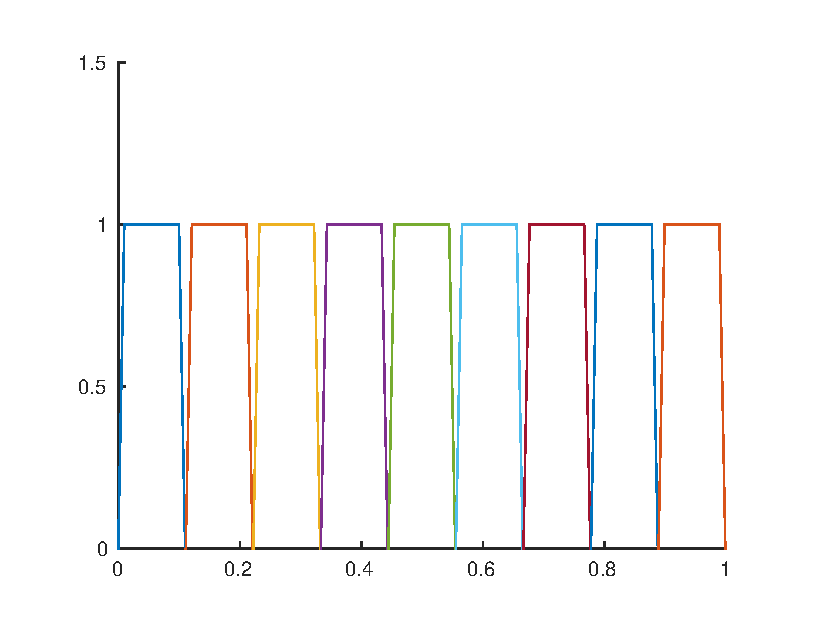
\includegraphics[width=\linewidth]{Pictures/basisconstant}
  \subcaption{B-spline basis for $p=0$}
  \label{fig:bspline_basis_constant}
\end{subfigure}%
\begin{subfigure}[b]{.3\linewidth}
  \includegraphics[width=\linewidth]{Pictures/basislinear}
  \subcaption{B-spline basis for $p=1$}
  \label{fig:bspline_basis_linear}
\end{subfigure}
\begin{subfigure}[b]{.3\linewidth}
  \includegraphics[width=\linewidth]{Pictures/basisquadratic}
  \subcaption{B-spline basis for $p=2$}
  \label{fig:lognorm_quadratic}
\end{subfigure}
\caption{B-spline basis functions, of degree $p=0$ (left), $p=1$ (middle) and $p=2$ (right).}
\label{fig:bsplineBases}
\end{figure}


By giving each of these basis functions a weight $\omega_i$ and normalizing them at each point by dividing by the total sum, we get the rational basis functions. Writing them out explicitly, in terms of B-spline basis functions $N_{i,p}$, the $n^{\text{th}}$-degree NURBS surface with $k$ control points $P_i$ is finally given by:
\begin{equation}
\label{eq:nurbscurve}
\vec{C}(u) = \frac{\sum_{i=1}^{k}N_i^n\left(u\right)\omega_{i}\vec{p}_{i}}{\sum_{i=1}^{k}N_i^n\omega_{i}}.
\end{equation}

B-splines have the following properties, which are useful for our problem:
\begin{itemize}
\item Degree $n$ and number of control points $\vec{P}_{i\cdots m}$ are independent.
\item B-Splines only change locally (depending on the degree $n$) when a control point is changed.
\end{itemize}

Analogous to the tensor product \Bez curve surfaces (see \autoref{eq:bezsurface}), one can define tensor product B-spline or NURBS surfaces:
\begin{equation}
\label{eq:nurbssurface}
\vec{S_\text{NURBS}}(u,v)=\frac{\sum\limits_{i=0}^n \sum\limits_{j=0}^m N_{i}^n(u) N_{j}^m(v) \omega_{i,j}\vec{p}_{i,j}}{\sum\limits_{i=0}^n \sum\limits_{j=0}^m N_{i}^n(u) N_{j}^m(v) \omega_{i,j}},
\end{equation}
where the case with all $\omega_{i,j} = 1$ corresponds to a B-Spline surface; respectively a NURBS surface if any $\omega_{i,j} \neq 1 $. With varying degrees and number of control points, these can be made to fit a variety of shapes. However, as the parameters $u$ and $v$ define a square in their two-dimensional parameter domain, there is a limit to what topologies may be realized with just one such NURBS surface. For example, an open cylinder could be constructed by one such surface where one of the sides meets its own beginning, whereas something with multiple holes - like a double torus, or a non-flat 8-shaped surface, would be impossible. Therefore, when using NURBS, surfaces are most often modelled using a network of connected patches. \todointern{maybe should include an example picture here} For more information about NURBS, see \cite{farin1999nurbs}.




		
		
		% ---------------------------------------------------------------------------
		%
		% Implementation 
		%
		% ---------------------------------------------------------------------------
		\chapter{Implementation}
		\label{chapter:Implementation}		
		% change chapter/section/part names as pleaseth thee!
%
% possibly later split into software pipeline/nurbs algorithms part!
%\section{Introduction to the software pipeline}
%not written yet

%<<<<<<< HEAD
%\section{From CAD to Voxels {\it has to be rewritten}}
\label{sec: CADToVoxels}
\section{From \acs{CAD} Model to Voxel Representation}
\label{sec: CADToVoxels}
Converting the CAD input to ToPy input along with all the boundary conditions is the first problem that needs to be addressed in our pipeline. The procedure has been described in four sections: the first section explains the logic behind specifying boundary conditions using a CAD software. Subsequent sections then talk about what the code does with this CAD input. The second section explains the extraction of different boundaries from the CAD geometry with extensive use of the OpenCascade C++ library. This is followed by two more sections on voxelization and writing of the output file. Finally, the last section explains the input file format for ToPy, and describes its operation. \autoref{fig:umlCADToVoxel} shows an overview of the structure of the code used for this part of the pipeline.

\begin{figure}[H]
\begin{center}
  \includegraphics[scale=0.5]{Pictures/CADToVoxel/UML_Complete_PNG.png}
\caption{UML diagram of the pipeline from CAD to a voxelized output. Many sections of the code use data-structures and algorithms from OpenCascade\cite{OpenCascade}.}
\label{fig:umlCADToVoxel}
\end{center}
\end{figure}

\subsection{Specification of Boundary Conditions for the Input Geometry}
\label{sec: GeomCreation}

\todo[inline]{Saumi: Here we describe what one needs to do in FreeCAD to set the loads, fixtures, and passive elements for the geometry. We also instruct the user to save the geometry as both IGES and STEP, and explain the reason for this.}


\subsection{Face Extraction and Categorization}
\label{sec: FaceExtraction}

%\tododone[inline]{}
Apart from using CADO directly, one can also call the face extraction step manually. For that, once the user has created their input geometry and saved it as STEP and IGES files, they can begin the execution by invoking the bash script \lstinline|CADTopOp.sh| located in \lstinline|/CADORoot/CADO/CPP|. For example, for a case located in directory \lstinline|/newuser/CADRoot/TestCase/| with file name \lstinline|geom|, force scaling factor of 240.19 and a refinement level of 2, the appropriate command to invoke the script from its folder would be: \\

\lstinline|$ ./CADTopOp.sh /CADRoot/TestCase/ geom 240.19 2| \\

The bash script basically invokes \lstinline|CADToVoxel| that parses the geometry, sorts out the faces based on their type, voxelizes the assembly, and writes the input for the topology optimizer. The script then calls the topology optimizer with this file as input. Once optimised, the script requests an extracted surface from the density voxel grid from the dual contouring algorithm. 

%It is worth noting, that as of the second milestone an integrated pipeling is available from the geometry input to the surface extraction through dual contouring. Connection with the next part of the pipeline is the objective for the third phase.

Here is an explanation of how the faces are extracted from the CAD input and how they are categorised based on the color:

\begin{enumerate}
	\item An instance of \lstinline|Reader| is created with the CAD source directory and file name as input. \lstinline|Reader| wraps the OpenCascade classes for reading STEP and IGES files into a single class, reads the two files, and holds them in two handles. Also \lstinline|Reader| instances are created for the non-changing domain and load file input.
	\item The \lstinline|ColorHandler| class takes over the handles from \lstinline|Reader|. \lstinline|ColorHandler| provides methods, each of which returns a list of faces (see \autoref{fig:umlCADToVoxel}). Depending on which method is called the returned list contains groups of fixtures, loads, passive faces, or all faces of the body.
	\item Each of the methods mentioned above internally calls the hidden function \lstinline|findColoredFaces()|. This method takes as input a color, and returns all faces that match it. It also takes as input a boolean variable \lstinline|isLoadSeeked| - if true, then the function returns all faces with load on them, and also a vector of the corresponding loads.
	\item The load vector is then scaled with respect to the scaling factor provided as input by the user.
\end{enumerate}

Once these face lists are available, they can be voxelized.


\subsection{Voxelization}
\label{sec: Voxelization}

\todointern[inline]{Severin: Describe the voxelization process. Explain concept of refinement.}
%what is voxelisation
As pointed out in section \ref{sec:ToPy} a very common formulation of topology optimization deals with regions that are specified as filled or empty. The minimum compliance problem is then solved on a discretized grid; the most common one is a volume raster in the form of cubes - so called voxels. Since ToPy requires a voxel grid in their input format, the next step is to render the geometry with a 3D raster of voxels.  

As described in the previous section, the geometry shape and faces for each boundary condition type, are stored in OpenCascade through the internal data type \lstinline|TopoDSShape|. As one can see in the UML Diagram \ref{fig: umlCADToVoxel} the \lstinline|voxelise| function is called internally by \lstinline|CADTOVoxel| -- for the shape and each faces separately. The voxelisation is then performed as follows: 
\begin{enumerate}
\item In order to combine the 3D voxel raster consistently, a bounding box is introduced.
\item In each dimension $2^n*l_d$ voxels are created, where $n$ is the user specified refinement level and $l_d$ is the size of the bounding box in the respective dimension $d$
\item Voxelization is performed with the OpenCascade  \lstinline|Voxel_FastConverter.hxx| class creating a \lstinline|VoxelShape|
\end{enumerate}
\todointern[inline]{OpenCascade TopoBoolDS shape}



%\subsection{Construction of ToPy Input File}
\label{sec: ToPyInputConstruction}

\todo[inline]{Severin: Explain the difference in the coordinate system of ToPy. Explain the mirroring of directions being done in the ToPyWriter.}



%\input{chapters/ImplementationSections/CADImpl/TopOpt}

 %In the end, to voxelize a file given as .stl-input, we could just call 
%\begin{lstlisting}
%~/Path/To/CVMLCPP/bin/voxelize ./<stl_file>.stl <voxelSize>
%\end{lstlisting}
%where $\mathtt{<voxelSize>}$ is an integer declaring the size of a voxel. 


\section{\it Boundary conditions}
=======
\todo[inline]{comment on the content of this chapter like at the beginning in other chapters}

\todo[inline]{this chapter covers the interfaces and application of the theory from the last chapter}

\todo[inline]{Explain why we need two files, reading two input files, color mapping. Voxelise Faces seperately, e.g. with flow chart. Or shift this to appendix?}


%\section{From \acs{CAD} Model to Voxel Representation}
\label{sec: CADToVoxels}
Converting the CAD input to ToPy input along with all the boundary conditions is the first problem that needs to be addressed in our pipeline. The procedure has been described in four sections: the first section explains the logic behind specifying boundary conditions using a CAD software. Subsequent sections then talk about what the code does with this CAD input. The second section explains the extraction of different boundaries from the CAD geometry with extensive use of the OpenCascade C++ library. This is followed by two more sections on voxelization and writing of the output file. Finally, the last section explains the input file format for ToPy, and describes its operation. \autoref{fig:umlCADToVoxel} shows an overview of the structure of the code used for this part of the pipeline.

\begin{figure}[H]
\begin{center}
  \includegraphics[scale=0.5]{Pictures/CADToVoxel/UML_Complete_PNG.png}
\caption{UML diagram of the pipeline from CAD to a voxelized output. Many sections of the code use data-structures and algorithms from OpenCascade\cite{OpenCascade}.}
\label{fig:umlCADToVoxel}
\end{center}
\end{figure}

\subsection{Specification of Boundary Conditions for the Input Geometry}
\label{sec: GeomCreation}

\todo[inline]{Saumi: Here we describe what one needs to do in FreeCAD to set the loads, fixtures, and passive elements for the geometry. We also instruct the user to save the geometry as both IGES and STEP, and explain the reason for this.}


\subsection{Face Extraction and Categorization}
\label{sec: FaceExtraction}

%\tododone[inline]{}
Apart from using CADO directly, one can also call the face extraction step manually. For that, once the user has created their input geometry and saved it as STEP and IGES files, they can begin the execution by invoking the bash script \lstinline|CADTopOp.sh| located in \lstinline|/CADORoot/CADO/CPP|. For example, for a case located in directory \lstinline|/newuser/CADRoot/TestCase/| with file name \lstinline|geom|, force scaling factor of 240.19 and a refinement level of 2, the appropriate command to invoke the script from its folder would be: \\

\lstinline|$ ./CADTopOp.sh /CADRoot/TestCase/ geom 240.19 2| \\

The bash script basically invokes \lstinline|CADToVoxel| that parses the geometry, sorts out the faces based on their type, voxelizes the assembly, and writes the input for the topology optimizer. The script then calls the topology optimizer with this file as input. Once optimised, the script requests an extracted surface from the density voxel grid from the dual contouring algorithm. 

%It is worth noting, that as of the second milestone an integrated pipeling is available from the geometry input to the surface extraction through dual contouring. Connection with the next part of the pipeline is the objective for the third phase.

Here is an explanation of how the faces are extracted from the CAD input and how they are categorised based on the color:

\begin{enumerate}
	\item An instance of \lstinline|Reader| is created with the CAD source directory and file name as input. \lstinline|Reader| wraps the OpenCascade classes for reading STEP and IGES files into a single class, reads the two files, and holds them in two handles. Also \lstinline|Reader| instances are created for the non-changing domain and load file input.
	\item The \lstinline|ColorHandler| class takes over the handles from \lstinline|Reader|. \lstinline|ColorHandler| provides methods, each of which returns a list of faces (see \autoref{fig:umlCADToVoxel}). Depending on which method is called the returned list contains groups of fixtures, loads, passive faces, or all faces of the body.
	\item Each of the methods mentioned above internally calls the hidden function \lstinline|findColoredFaces()|. This method takes as input a color, and returns all faces that match it. It also takes as input a boolean variable \lstinline|isLoadSeeked| - if true, then the function returns all faces with load on them, and also a vector of the corresponding loads.
	\item The load vector is then scaled with respect to the scaling factor provided as input by the user.
\end{enumerate}

Once these face lists are available, they can be voxelized.


\subsection{Voxelization}
\label{sec: Voxelization}

\todointern[inline]{Severin: Describe the voxelization process. Explain concept of refinement.}
%what is voxelisation
As pointed out in section \ref{sec:ToPy} a very common formulation of topology optimization deals with regions that are specified as filled or empty. The minimum compliance problem is then solved on a discretized grid; the most common one is a volume raster in the form of cubes - so called voxels. Since ToPy requires a voxel grid in their input format, the next step is to render the geometry with a 3D raster of voxels.  

As described in the previous section, the geometry shape and faces for each boundary condition type, are stored in OpenCascade through the internal data type \lstinline|TopoDSShape|. As one can see in the UML Diagram \ref{fig: umlCADToVoxel} the \lstinline|voxelise| function is called internally by \lstinline|CADTOVoxel| -- for the shape and each faces separately. The voxelisation is then performed as follows: 
\begin{enumerate}
\item In order to combine the 3D voxel raster consistently, a bounding box is introduced.
\item In each dimension $2^n*l_d$ voxels are created, where $n$ is the user specified refinement level and $l_d$ is the size of the bounding box in the respective dimension $d$
\item Voxelization is performed with the OpenCascade  \lstinline|Voxel_FastConverter.hxx| class creating a \lstinline|VoxelShape|
\end{enumerate}
\todointern[inline]{OpenCascade TopoBoolDS shape}



%\subsection{Construction of ToPy Input File}
\label{sec: ToPyInputConstruction}

\todo[inline]{Severin: Explain the difference in the coordinate system of ToPy. Explain the mirroring of directions being done in the ToPyWriter.}



%\input{chapters/ImplementationSections/CADImpl/TopOpt}

 %In the end, to voxelize a file given as .stl-input, we could just call 
%\begin{lstlisting}
%~/Path/To/CVMLCPP/bin/voxelize ./<stl_file>.stl <voxelSize>
%\end{lstlisting}
%where $\mathtt{<voxelSize>}$ is an integer declaring the size of a voxel. 

%>>>>>>> 75c6f5bc947f0a0353c0ae26deaec8dd0bdc19c0

Due to the good range of topology optimization software available, we decided to adapt an open-source topology optimizer to our needs, \emph{ToPy}.

\subsection{ToPy library}\label{sec:ToPy}
ToPy \cite{ToPy} is a python library/program, written by William Hunter and documented in \cite{Hunter2009}, implementing the SIMP model and method described in \autoref{subsec:TopOpTheory}. It is based on the 99-line Matlab code by Sigmund's for minimum compliance \cite{sigmund200199}. The program can optimize the three above named problem types, minimum compliance, heat conduction and mechanism synthesis-- in 2D as well as 3D. It uses available open source python software, as for example Pysparse and Numpy, leading to improved speed, porta- and scalability. The whole program is steered by an input file which-- with the help of the documentation-- is straightforward to use and easy to adapt. 

\subsection{Implementation}%TODO: MOVE TO AN IMPLEMENTATION SECTION
In terms of our implementation, we use ToPy as a blackbox topology optimizer. This means, we launch the program with an input file based on our scenario, let ToPy run and proceed by working with the output of ToPy. The intention is to touch the solver itself as less as possible to be able to just plug in different solvers later on. Implementation-wise that means, that we wrote a program which takes as input a voxelized CAD design in, for example, stl-format and outputs a tpd-file which can be used by ToPy. Results of the process can be seen in figure \ref{fig: topyStar}. Here, a star was given as input from a stl-file. We fixed the voxels in the corners of the structure, while we set a load in the middle, pointing into the structure. As can be seen, the optimization process "cuts" away unnecessary material in-between the corners and even in the middle of the material and returns stiff structure for a minimal amount of material. 
\begin{figure}
\centering
\begin{subfigure}{
  \includegraphics[width=.2\linewidth]{Pictures/TopOp/Star_Optimized0_Trans.png}}
\end{subfigure}%
\begin{subfigure}{
  \includegraphics[width=.2\linewidth]{Pictures/TopOp/Star_Optimized2_Trans.png}}
\end{subfigure}
\begin{subfigure}{
  \includegraphics[width=.2\linewidth]{Pictures/TopOp/Star_Optimized4_Trans.png}}
\end{subfigure}
\begin{subfigure}{
  \includegraphics[width=.2\linewidth]{Pictures/TopOp/Star_Optimized5_Trans.png}}
\end{subfigure}
\caption{Topology Optimization with minimum compliance of a star structure, given by an stl-file. The fixtures were applied in the corners of the star, while a load was set in the middle.}
\label{fig: topyStar}
\end{figure}

As was mentioned above, surface extraction is an intermediate step after Topology Optimization and NURBS representation in order to facilitate the conversion. In terms of implementing the surface extraction, we used VTK.

%\subsection{VTK Toolbox}


%The VTK toolbox was used in order to implement the algorithms on our optimized data. It is a heavily object
%oriented toolbox. Our first approach was to use the built in Marching Cubes algorithm,
%nevertheless it did not work with our unstructured grid data. It just works for ImageData and
%PolyData . For structured and unstructured grids the tool to render the isosurface is the \textit{Contour Filter} tool. Unfortunately the documentation does not present which algorithm the tool uses. It
%can be inferred that it is an extended Marching cubes algorithm.

The VTK Toolbox is an open--source tool, providing algorithms for "3D computer graphics, image processing, and visualization" \cite{VTKToolbox}. Among the variety of tools, VTK offers algorithms that allow us to obtain a surface representation from voxel data. Among these algorithms, we could find Marching Cubes, Dual Contouring and also a decimation tool, which is useful for reducing the data size further for the NURBS-representation step.


%\subsection{Implementation}
The \textit{Marching Cubes} algorithm is inapplicable to our case of unstructured grid data, since it only works with ImageData and PolyData, which are the main data types in VTK. For structured and unstructured grids the tool to render the isosurface is the \textit{Contour Filter} tool. Unfortunately, the documentation does not present which algorithm the tool uses. It can be inferred that it is an extended \textit{Marching Cubes} algorithm.
The \textit{Contour Filtering} works fine but the visualization of our data was still not possible
and an intermediate step was needed. We used the \textit{Implicit Modelling} tool which is a filter that
computes the distance from the input geometry to the points of an output structured point set.
This distance function can then be "contoured" to generate new, offset surfaces from the original
geometry. Although this approach allowed the visualisation, some crucial information was lost. In particular, holes are not represented in the final model.  


\begin{figure}
\centering
   \scalebox{0.4}{\includegraphics{Pictures/contouring.pdf}}\\
   \caption{Contour Filtering tool after Implicit Modelling}
   \label{fig:contouring}
\end{figure}

A further idea to solve this problem is to first convert the volume data into point data
and only then present it to the \textit{Contour Filtering} tool (\autoref{fig:contouring}).

In order to reduce computational costs of the following \textit{NURBS fitting} process, presented in the next section, we need to create a coarser mesh from the fine one. The number of triangles that represent the
isosurface can be reduced with the \textit{decimation} tool.  VTK has the
decimation tool which works for 3D triangle data. A smoothing step is necessary in between
to get the new connections right. The top part of figure \ref{fig:Decimation} shows a 50 \% reduction of the
triangles, a noticeable difference can not be perceived. On the lower part a 90 \% reduction is
obtained, it is nevertheless still difficult to see a difference. Triangle meshes can be easily
coarsened since there are many open source algorithms that reduce the number of triangles.

\begin{figure}
\centering
   \scalebox{0.4}{\includegraphics{Pictures/Decimation.pdf}}\\
   \caption{Decimation of triangles. \textit{Top:} 50\% \textit{Lower:} 90\%}
   \label{fig:Decimation}
\end{figure}


\section{From extracted surface to NURBS representation: an algorithmic journey}
As of yet, there is no open-source software which provides the conversion from a \textit{mesh-based} geometry to NURBS representation. Hence, one of the main challenges of both the algorithmic and implementation part of this project is to develop one from scratch. Due to a variety of possible approaches to tackle this problem (e.g. \cite{becker2011advanced},\cite{eck1996automatic}), we have conducted a profound prototyping work. In order to avoid a cumbersome and time-consuming implementation overheads during the prototyping phase, we have used MATLAB \cite{MATLAB}. Once the algorithms to be used are finalized, the prototypes are to be implemented using a non-proprietary language, such as Python or C++.
\subsection{Fitting pipeline}
\begin{figure}
\centering
  \includegraphics[width=.85\linewidth]{Fitting_workflow.png}
  \caption{NURBS fitting pipeline}
  \label{fig:fitting_pipeline}
\end{figure}
Since the geometry obtained after topology optimization can be arbitrary complex, we might not be able to find a good fit using only one patch. We seek a multi step algorithm, allowing us to break the overall big problem into smaller problems, which can be handled relatively easy.
Based on the algorithm described in \cite{eck1996automatic}, our overall fitting pipeline looks as follows (see \autoref{fig:fitting_pipeline}):
\begin{itemize}
	\item Patch selection (breaking our problem in small pieces which can be solved using least squares)
	\item Parametrization of obtained patches
	\item B-spline fitting using least squares
	\item Smooth connection of patches
	\item Conversion back to CAD
\end{itemize}

The pipeline given above, once implemented, will provide us with a flexible algorithm for converting an arbitrary complex mesh based geometry into NURBS and, hence, CAD-representation.
\subsection{Processing parametrized points}
\subsection{Applying Peters' scheme}




%how the algorithms were implemented



		
		% ---------------------------------------------------------------------------
		%
		% Implementation 
		%
		% ---------------------------------------------------------------------------
		\chapter{Summary \& discussion\todo{better caption?}}
		\label{chapter:Discussion}		
		\chapter{Summary and future work}
\todourgent[inline]{how should we structure this?}

\section{In a Nutshell:\ \acl{CADTopOpt}}
\label{sec:nutshell}
\todourgent[author=Benni]{@ Erik: please proofread! Especially discussion or results.}
\todourgent[author=erik]{@Erik:maybe talk a bit more about summary of the report?}
In this report, we present CADO, Computer Aided Design Optimizer, which is the result of this project. In summary, CADO works as a fully integrated tool-chain from the CAD input file to an optimized CAD file. First, the input geometry undergoes voxelization using OpenCASCADE to ensure compatibility with the topology optimizer. Second, the topology is optimized by employing the open-source tool ToPy \cite{ToPy}.  
Next, a two-stage Dual Contouring surface reconstruction scheme is executed on the output of topology optimization. This gives us coarse parametrization patches and fine vertices as output.
A B-Spline surface is then fitted through this data by a least-square approach using control points described by the Peters' scheme \cite{peters1992constructing} in order to ensure continuous and smooth surfaces. Lastly, a FreeCAD macro script performs boolean operations to enforce geometric constraints and exports the geometry to a standardized CAD file \cite{FreeCAD}.
Note that intermediate steps can be replaced in the future with more suitable solutions. 

The functionality of the tool was tested through three test cases described in \autoref{sec:tests}. We made the following observations:
\begin{itemize}
\item The design problem could be easily formulated in the form of CAD files.
\item The CAD files were parsed to construct the topology optimization problem. Only small problems (Bridge, Cantilever) could be handled using ToPy. For bigger problems (GE Jet Engine Bracket) ToPy was not sufficient.
\item Smooth NURBS surfaces of arbitrary topology were successfully reconstructed from the optimization solution, albeit with a high number of patches. Deformations of the resulting NURBS surfaces were observed ("dents" in the bridge). The reason for this is limited accuracy in the projection scheme described in \autoref{sssec:projection}. Additionally, conservation of topological features was not guaranteed (GE Jet Engine Bracket).
\item Finally, after post-processing for geometry constraints, the result was exported as a standard CAD \emph{.step} file.
\end{itemize}
CADO is a strong proof of concept for CAD integrated topology optimization. It solved the proposed test scenarios to a qualitative level of satisfaction. Nevertheless, CADO's maturity to a full-fledged software package for engineering problems requires further improvements and additions.

\section{Future Work}
\label{sec:Future}
\todourgent[inline, author=Benni]{avoid subsections! Just show up problems and outlook to literature: no pictures, no explanations!}
\begin{enumerate}
\item Avoid special manifold treatment, find a general approach (refer to manifold DC paper)
\item Alternative approach: Isogeometric analysis?
\item Adaptive DC
\item Adaptive Peters' scheme
\item faster Topology Optimization
\item Improved Parameter estimation (w.r.t. accuracy and speed)
\item error estimates (DC, Peters' scheme, Topology Optimization)
\item Postprocess shape optimization?
\end{enumerate}
\subsection{Surface reconstruction}
\todointern[inline]{proofreading!}
Our implementation of the surface reconstruction scheme explained in \autoref{ssec:reconstruction} and the two-scale approach described in \autoref{ssec:parametrization} yet only work for very simple structures like spheres or tori. For more complicated structures -- for example the output of a topology optimization tool -- we either have to use a very high resolution, or we have to apply certain optimizations, which will be explained in the following.

\subsubsection{More flexible dual contouring}
\todointern[inline]{content!}

\subsubsection{Dual Marching Methods}
\todointern[inline]{Benni:Proofreading!}
In \autoref{sec:surfaceBackg} we have introduced \ac{MC} and \ac{DC} and discovered that both methods have certain drawbacks:
\begin{itemize}
\item \ac{MC} always produces manifold surfaces and resolves ambiguities correctly, while \ac{DC} does not have this property.
\item \ac{DC} has the ability to produce \ac{quad} surfaces and preserve sharp features, while \ac{MC} produces surfaces consisting of \acp{tri}\footnote{The construction of \acp{tri} is not a drawback of the \ac{MC} method in general, but for our purpose we have to construct \acp{quad} and therefore this point is crucial. If we want at the end to produce a \ac{NURBS} surface, we have to rely on \acp{quad}, because \ac{NURBS} have a rectangular topology. \Acp{tri} just do not fit the topology of \ac{NURBS}. Further explanation can be found in \autoref{sec:NURBS} and \autoref{sec:surfaceImpl}} and sharp features are often lost.
\end{itemize}
To come up with these drawbacks, hybrid methods have been developed. These methods use ideas from both the \ac{MC} and the \ac{DC} approaches (For a short summary of those ideas see \autoref{tab:dualmarching}).
\begin{table}[H]
\begin{tabularx}{\textwidth}{X|X}
\multicolumn{1}{c|}{\acl{MC}} 
    & \multicolumn{1}{c}{\acl{DC}} 
\\
\hline
\begin{itemize}[ topsep = 0pt, leftmargin=1em]
\item traverse voxels and use a look up table for the creation of faces
\item creates manifold and ambiguity free surfaces
\end{itemize}
&
\begin{itemize}[ topsep = 0pt, leftmargin=1em]
\item place vertices inside voxel\footnote{Determine positions by -- for example -- minimizing \autoref{eq:QEF}.}
\item construct \acp{quad} by joining vertices in voxels with a common edge
\end{itemize}
\end{tabularx}
\caption{ideas from \ac{DC} and \ac{MC} contributing to dual marching methods.}
\label{tab:dualmarching}
\end{table}
In the following we will briefly introduce two of those hybrid methods:

\begin{itemize}
\item \textbf{\acl{DualMC}}:
The \acf{DualMC} method is --- like already stated above --- a hybrid of \ac{MC} and \ac{DC}: We traverse the cubes like in \ac{MC} and insert vertices and connect them like in \ac{DC}. The combination of the $256$ different cases from the basic \ac{MC}, the extension for creating ambiguity free surfaces and the framework of \ac{DC} results in a very effective but also complex algorithm. A drawback of this method is that for certain configurations we have to create non-\ac{quad} faces --- especially faces with odd number of vertices are difficult to convert to \acp{quad}, if one wants to obtain a \ac{quad}-only surface like in \ac{DC}. We refer the interested reader to  \cite{Nielson2004, Zhang2012}.

\begin{figure}
\begin{center}
\includegraphics[width = .5\textwidth]{Pictures/SurfaceReconstruction/MCtoDualMC.png}
\end{center}
\caption{How one of the \ac{MC} cases is treaten in \ac{DualMC} algorithm (figure from \cite{Nielson2004})}
\end{figure}

\item \textbf{\acl{DualMT}}:
While \ac{DualMC} is a very complicated algorithm, \acf{DualMT} uses tetrahedra instead of cubes and therefore reduces the $256$\footnote{With a proper treatment of ambiguities we get even more than those $256$ cases.} different cases from \ac{MC} to $2^4=16$ cases. Furthermore a treatment of ambiguous cases is not necessary anymore, since there are no ambiguous cases for this method\todointern{really? check this or find reference!}.
Even though the method is working on tetrahedra, we can still apply it to a voxel dataset, by composing each cube out of 5 or 6 tetrahedra (\autoref{fig:splittingCubes}). Nevertheless, this high amount of simplification comes with a drawback: The treatment of ambiguous cases depends on the splitting scheme applied to a cube\todointern{proof or reference! Show 2D example.}. Further detail on this method can be found in \cite{Nielson2008}.

\begin{figure}
\begin{center}
\includegraphics[width = .5 \textwidth]{Pictures/SurfaceReconstruction/SplittingCubes.png}
\caption{Two different subdivision schemes for cubes into tetrahedra (figure from \cite{Nielson2008})}
\label{fig:splittingCubes}
\end{center}
\end{figure}

\end{itemize}


		
		% ---------------------------------------------------------------------------
		%
		% Appendix
		%
		% ---------------------------------------------------------------------------
%		\part*{Appendix}
	%	\addcontentsline{toc}{part}{Appendix}
%		\appendix 
		
		%---------------------------------------
%		\chapter{Source Code}
%		\label{chapter:source}
%		
Here would be well-documented, nicely formatted source code.


\begin{lstlisting}[language={C++}, label={Hello World.}, frame = single ]
//include iostream for std::cout
#include<iostream>

//here beginneth the main function of the program.
int main(int argc, char * argv[])
{
	//output "Hello World" to the running terminal
	std::cout<<"Hello World!" << std::endl;
	
	//finish, returning no-error value 0.
	return 0;
}
dsgd
\end{lstlisting}
		
		%\chapter{Next Appendix}
		


  	\clearemptydoublepage
  
	\bibliography{bibliography/literature}
	
	\cleardoublepage
	\printacronyms[	include-classes=abbrev,
					name=Abbreviations,
					sort = true]

	\printacronyms[	include-classes=nomencl,
					name=Nomenclature,
					sort = true]
	
 
\end{document}

